%!TEX root=masterproef.tex

\chapter{Inleiding}
\label{inleiding}

Ofschoon de naam nog geen gemeengoed is, is de opmars van draadloze
sensornetwerken (DSN) in ons dagelijks leven niet meer te stoppen. Na de
revolutie van de persoonlijke computer, de smartphone en het tablet vinden nu
onafhankelijke, minuscule computers hun weg naar allerlei alledaagse dingen en
plaatsen in ons leven. Deze netwerken kunnen met hun sensoren de kleinste
wijzigingen in hun omgeving optekenen. Via een draadloos netwerk staan de
sensoren in verbinding met elkaar en de buitenwereld. Zo leveren ze hun
informatie af, waardoor wij op elk moment precies weten hoe warm het in elke
kamer van ons huis is of welke groenten nog in de koelkast liggen. Het lijkt
nog science fictie, maar deze toekomst is heel wat dichterbij dan we vermoeden.

Om deze technologie te omarmen en ons leven verder in te richten met deze
ondersteunende hulp, moeten we ons er van vergewissen dat deze technologie
betrouwbaar en veilig is. Als enkele sensoren in ons huis slechts een kleine
stap met weinig potenti\"ele, problematische gevolgen lijkt, moeten we ons toch
bezinnen en beseffen dat al deze kleine computers zeer interessante
inbraakmogelijkheden bieden aan anderen met minder positieve bedoelingen.

Misschien wil de concurrent van de producent van onze yoghurt zijn collega wel
in diskrediet brengen door er voor te zorgen dat onze slimme koelkast het
nalaat ons te verwittigen dat de yoghurt vervallen is. Misschien vindt de
gasleverancier het wel leuk om, wanneer we niet thuis zijn, de thermostaat een
graadje hoger te zetten.

De mogelijkheden van draadloze sensornetwerken lijken eindeloos en ze kunnen de
kwaliteit van ons leven ingrijpend veranderen. Ze mogen echter geen bijkomende
bedreiging introduceren. In deze masterproef duiken we in de wereld van
draadloze sensornetwerken en willen we nagaan of en hoe we deze kunnen voorzien
van bescherming tegen minder goede bedoelingen.

In dit eerste hoofdstuk introduceren we in sectie \ref{section:wsn} draadloze
sensornetwerken. Hoe zijn ze opgebouwd? Wat zijn de mogelijkheden en
beperkingen? In sectie \ref{section:beveiligen} verschuift de nadruk naar
beveiliging: Wat zijn de gevaren? Hoe kunnen deze vastgesteld worden? Hoe
kunnen sensorknopen beschermd worden?

Verder wordt in sectie \ref{section:probleem} het feitelijke probleem
gedefini\"eerd en wordt in sectie \ref{section:doelstelling} een doelstelling
voorgesteld. Na dit hoofdstuk liggen alle speelstukken op tafel.

\section{Draadloze sensornetwerken}
\label{section:wsn}

Sinds de late jaren '90 zijn draadloze sensornetwerken een bron geweest voor
een overvloed aan onderzoek. Binnen en buiten universiteiten werden deze
netwerken ingezet voor allerhande toepassingen: van het opvolgen van
microklimaten bij het telen van gewassen \citep{baggio2005wireless} tot het
vastleggen van vulkanische activiteit \citep{werner2005monitoring} en het
opvolgen van overstromingsgebieden \citep{hughes2006gridstix}.

Wat moeten we ons eigenlijk voorstellen bij een draadloos sensornetwerk? We
bekijken kort de sensorknopen, waarmee het netwerk wordt opgebouwd. Vervolgens
belichten we het draadloze netwerk dat de knopen in staat stelt om met elkaar
en met de buitenwereld te communiceren.

\subsection{Sensorknopen}

Sensorknopen zijn in essentie zeer eenvoudige computers. Ze worden typisch
opgebouwd rond een microcontroller (\mcu). Dit is een digitaal ontwerp dat
zowel een processor, als geheugen en invoer- en uitvoerkanalen bevat op \'e\'en
ge\"integreerde schakeling. Ze worden daarom ook wel \emph{systeem-op-een-chip}
(Engels: \emph{System-on-Chip}) (SoC) genoemd. Figuur \ref{fig:motes} toont
enkele typische sensorknopen.

\begin{figure}[ht]
\centering
\begin{subfigure}{.24\textwidth}
  \centering
  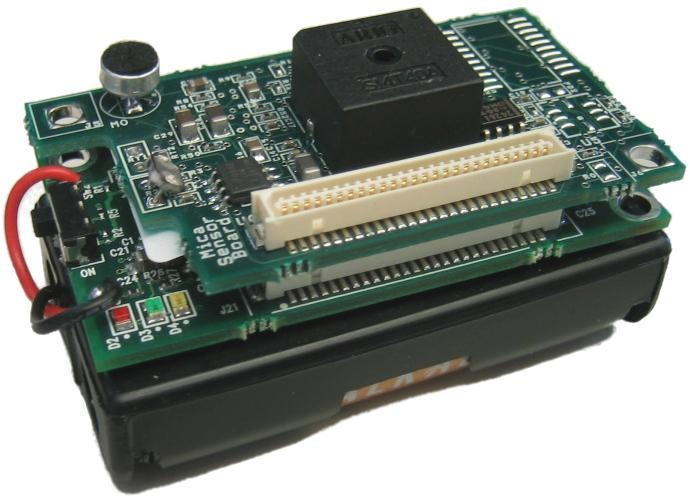
\includegraphics[width=.9\linewidth]{./resources/mica2.jpg}
  \caption{Mica2}
  \label{fig:mica2}
\end{subfigure}
\begin{subfigure}{.24\textwidth}
  \centering
  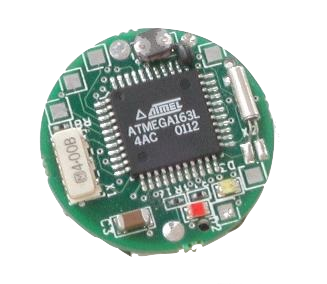
\includegraphics[width=.9\linewidth]{./resources/dot.png}
  \caption{Dot}
  \label{fig:dot}
\end{subfigure}
\begin{subfigure}{.24\textwidth}
  \centering
  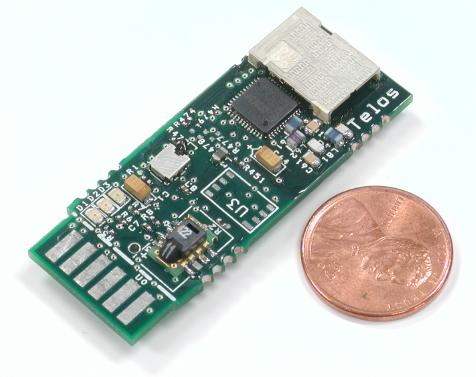
\includegraphics[width=.9\linewidth]{./resources/telos.jpg}
  \caption{Telos}
  \label{fig:telos}
\end{subfigure}
\begin{subfigure}{.24\textwidth}
  \centering
  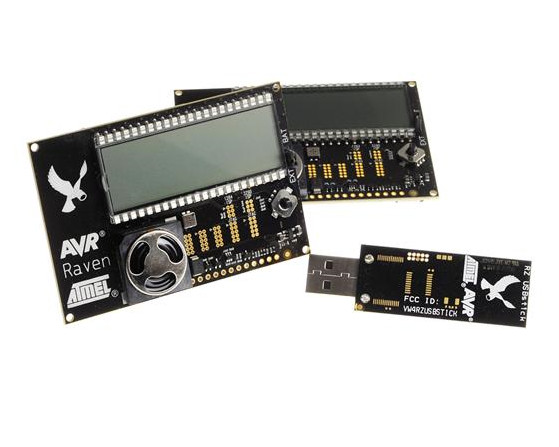
\includegraphics[width=.9\linewidth]{./resources/raven.jpg}
  \caption{AVRraven}
  \label{fig:raven}
\end{subfigure}
\caption{Voorbeelden van sensorknopen.}
\label{fig:motes}
\end{figure}

Naast de \mcu heeft een typische sensorknoop tevens een draadloze radio. Je kan
dit vergelijken met de Wi-Fi verbinding die je tegenwoordig in de meeste
computers of smartphones vindt. Voor sensorknopen wordt echter meestal
geopteerd voor een draadloze radio die een minimum aan energie probeert te
verbruiken. Verschillende nieuwe draadloze netwerkstandaarden zijn de laatste
jaren op de voorgrond getreden. De bekendste zijn 6LoWPAN \citep{rfc:6282} en
ZigBee \citep{alliance2012zigbee}. In de volgende paragrafen bekijken we ZigBee
van naderbij; enerzijds omwille van de toepassing in deze masterproef, maar ook
omwille van de voorbeeldfunctie die het kan aannemen voor deze groep van
draadloze standaarden.

\subsection{ZigBee}
\label{subsection:zigbee}

ZigBee zelf is een laag bovenop de netwerklaag gekend als IEEE 802.15.4
\citep{ieee2009802.15.4}. Deze voorziet standaarden op vlak van energiegebruik,
adressering, foutcorrectie, vormgeving van berichten \dots en vormt zo de
fundamenten voor zgn. \emph{low-rate wireless personal area networks}
(LR-WPAN). ZigBee voegt hieraan nog drie belangrijke eigenschappen toe:
routering, ad-hoc netwerk creatie en zelfherstellende maasnetwerken (Engels:
\emph{mesh networks}) \citep{oreilly2010buildingwsn}.

Een ZigBee netwerk wordt opgebouwd door knopen die elk \'e\'en van drie
verschillende functies kunnen innemen: co\"ordinator, router of eindknoop. Elk
netwerk heeft \'e\'en \emph{co\"ordinator}. Deze knoop is verantwoordelijk voor
het samenbrengen van het netwerk en definieert de eigenschappen, bv. met
betrekking tot de beveiliging.

Een \emph{router} stelt andere knopen in staat om met elkaar te communiceren.
Deze knopen zijn daarom meestal voorzien van een permanente stroomvoorziening,
omdat ze zich in tegenstelling tot \emph{eindknopen}, wegens hun
communicatieondersteunende rol, niet in een slaapstand kunnen zetten.

\emph{Eindknopen}, tot slot, kunnen zich louter verbinden met een netwerk, er
berichten via versturen en berichten voor zichzelf ontvangen. Het is niet de
bedoeling om berichten van andere knopen voor andere knopen door te sturen.
Typisch trachten ze ook hun energieverbruik te minimaliseren door hun draadloze
radio zoveel mogelijk uit te schakelen. Hierdoor worden ze op dat moment
onbereikbaar. Het is dankzij \emph{routers}, die berichten voor de
\emph{eindknopen} tijdelijk opslaan, dat ze toch berichten kunnen ontvangen.

\subsection{Netwerktopologie en -adressen}
\label{subsection:topologie}

Met knopen kunnen verschillende netwerktopologie\"en gebouwd worden. Figuur
\ref{fig:topologie} geeft een overzicht van de mogelijkheden. In zijn
eenvoudigste vorm bestaat een netwerk uit een co\"ordinator en een eindknoop.
Wanneer meerdere eindknopen verbonden zijn met dezelfde co\"ordinator, vormen
zij een stertopologie. Alle communicatie verloopt via de centrale
co\"ordinator. In een maasnetwerk, worden routers ingeschakeld om communicatie
via verschillende wegen mogelijk te maken. Eindknopen zijn verbonden met deze
routers of met de co\"ordinator. Routers en co\"ordinator kunnen berichten
ontvangen van eindknopen en deze versturen naar andere eindknopen, al dan niet
via andere routers. Een speciale vorm van een maasnetwerk is een clusterboom.
Hierbij vormen groepen van eindknopen en een router een cluster. De router is
verbonden met de co\"ordinator, eventueel opnieuw via andere routers, en zo
wordt een boomstructuur gevormd. De routers die de clusters van eindknopen
realiseren worden ook clusterhoofden genoemd.

\begin{figure}[ht]
  \centering
  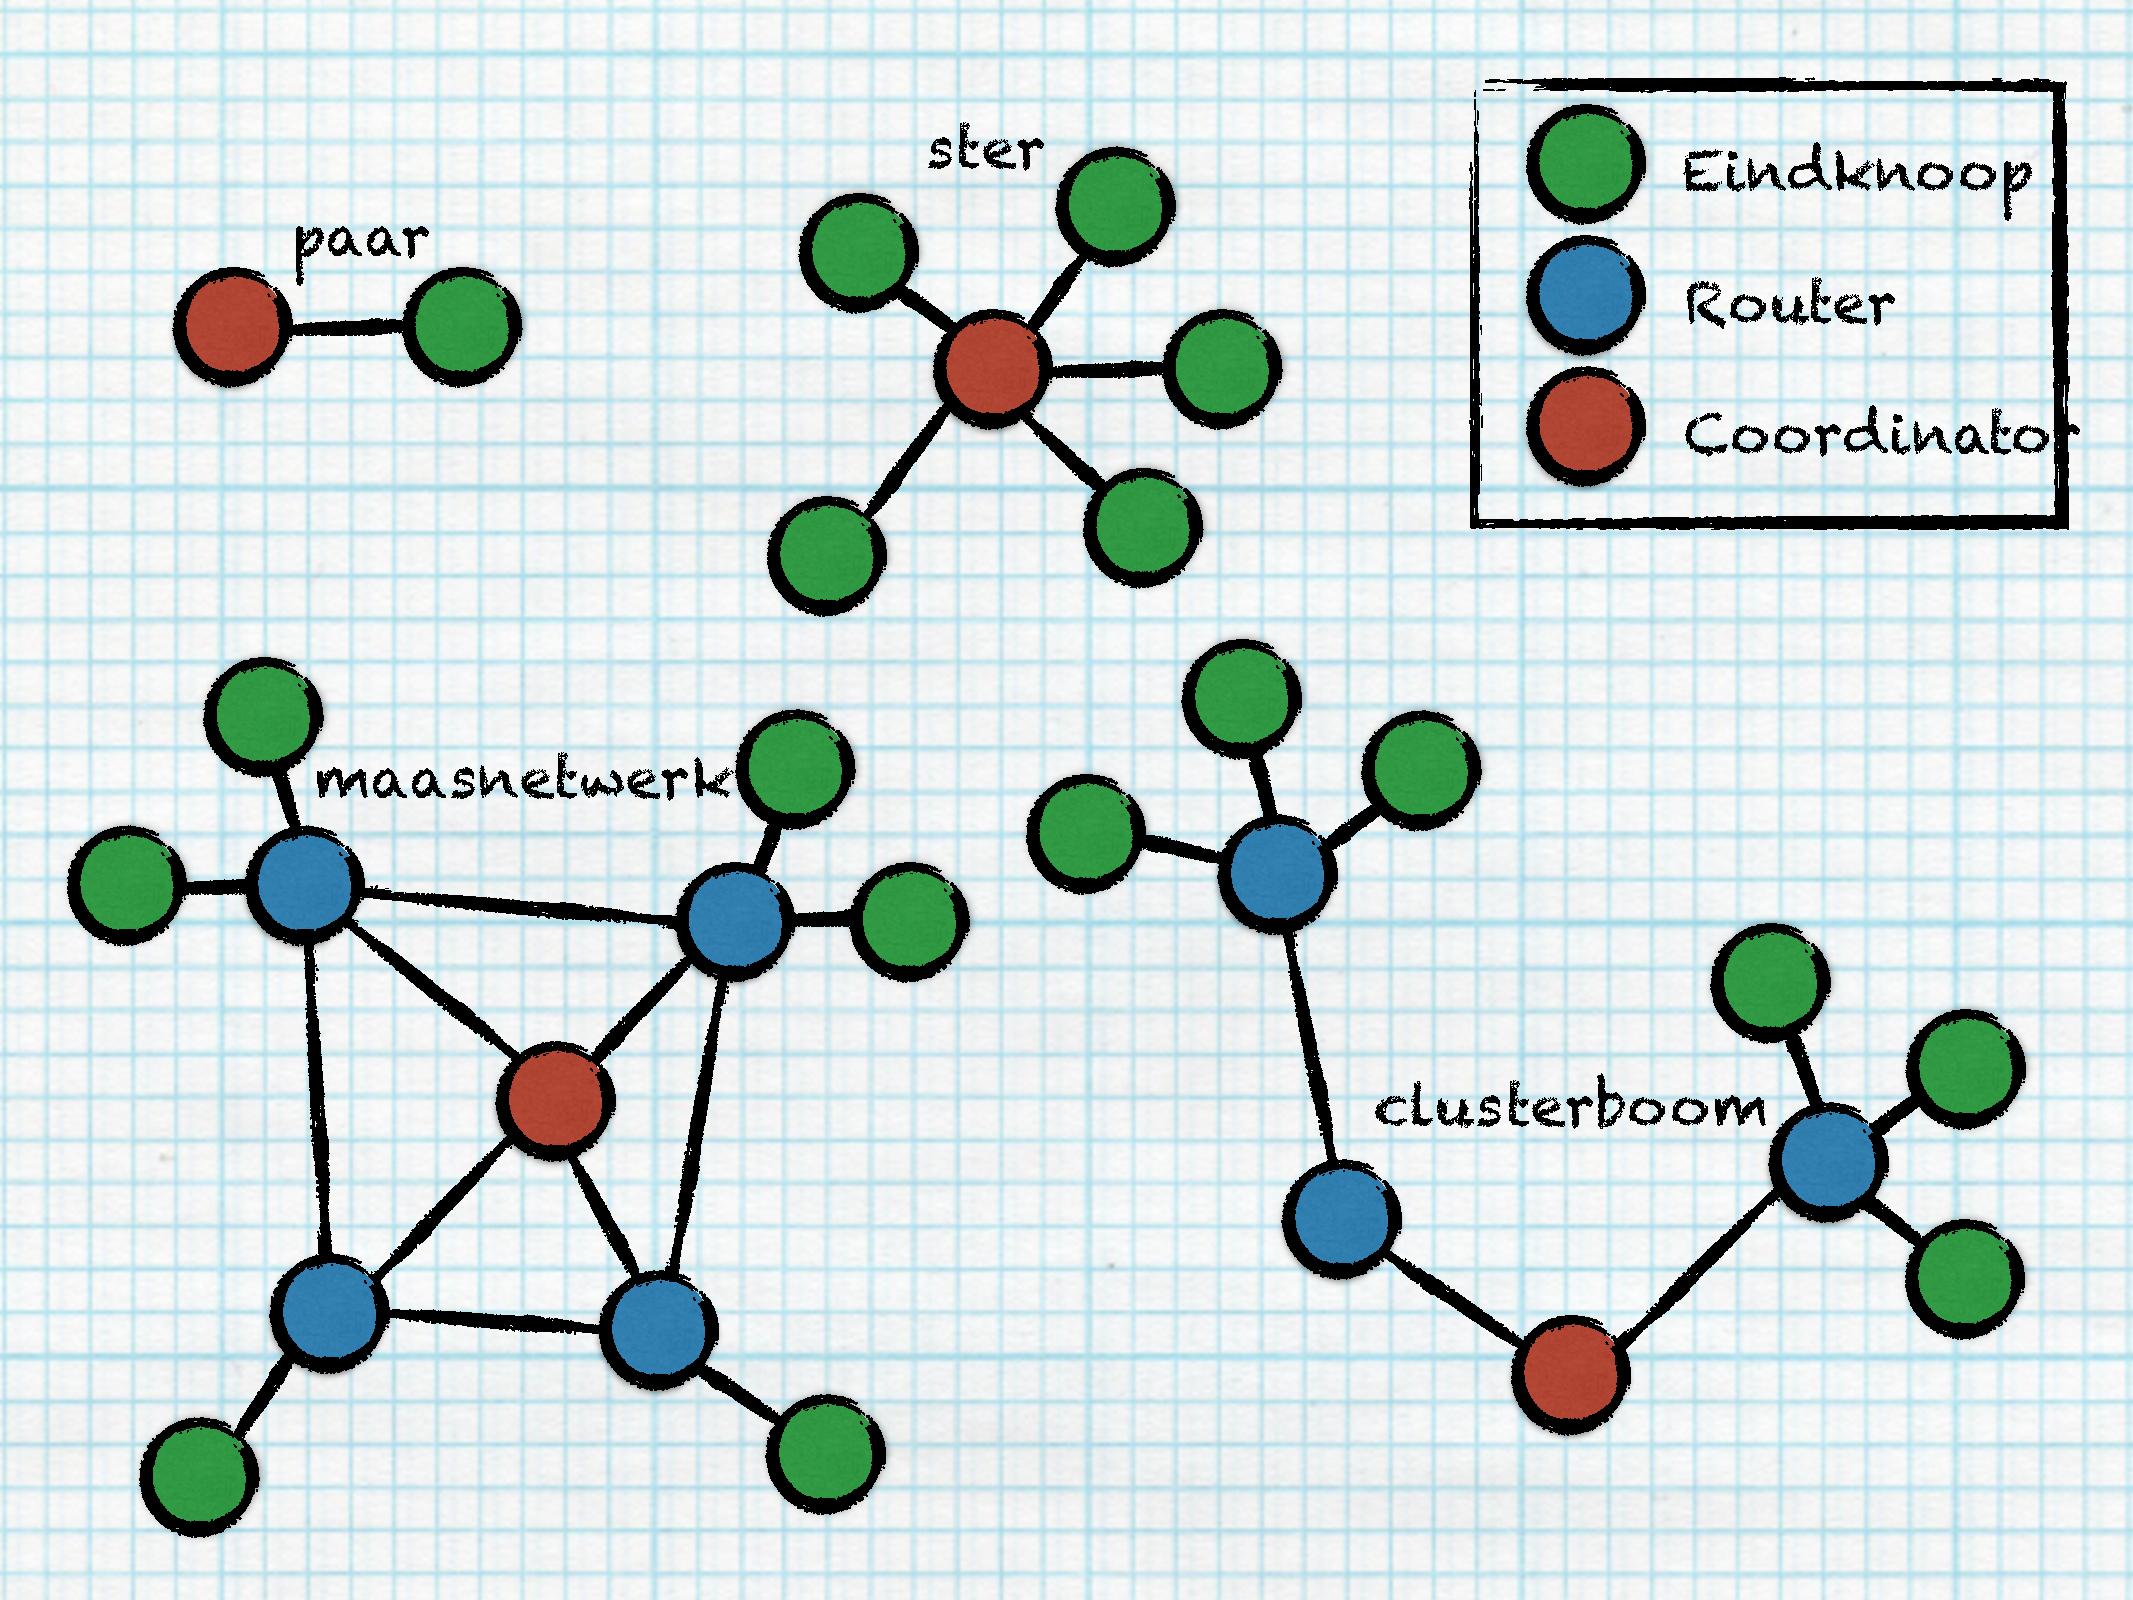
\includegraphics[width=0.7\linewidth]{resources/topology.pdf}
  \caption{Verschillende mogelijke netwerktoplogie\"en.}
  \label{fig:topologie}
\end{figure}

Het lijkt evident, maar elke knoop, in eender welke topologie, heeft een eigen,
uniek adres, eigenlijk meerdere. Zo heeft een ZigBee knoop een uniek adres
binnen het netwerk waaraan het deelneemt. Dit adres wordt door de co\"ordinator
van het netwerk toegekend aan een knoop wanneer deze toetreedt tot het netwerk.
Dit \emph{netwerk adres} bestaat uit 16 bits en laat dus toe om 65534 (uit
$2^{16} = 65536$) verschillende adressen toe te kennen. Het adres
\ttt{0x0000}\footnote{We hanteren voor de notatie van adressen de hexadecimale
voorstelling. Elk cijfer stelt een groep van 4 bits voor. 4 groepen stellen zo
een 16 bit adres voor.} reserveert de co\"ordinator voor zichzelf en het adres
\ttt{0xFFFE} wordt typisch gebruikt als het zgn. \emph{broadcast adres}, het
adres waarnaar een bericht gestuurd wordt dat bij alle andere knopen dient
afgeleverd te worden.

Daarnaast heeft elke ZigBee radio ook een adres dat gegarandeerd overal uniek
is. Dit bestaat uit 64 bits en wordt samengesteld uit twee delen: een eerste
deel beslaat de eerste 32 bits en is voorbehouden voor een unieke identificatie
van de producent. De volgende 32 bits is een uniek nummer binnen de productie
van de producent. Een netwerk zal veelal uit sensoren met dezelfde draadloze
radio's bestaan. Het is daarom logisch dat er gebruik gemaakt wordt van een
\emph{netwerk adres}, dat slechts 16 bits groot is en dus een aanzienlijke
besparing aan geheugen kan opleveren.

Naast de adressen van de knopen is er ook nog het zogenaamde \emph{personal
area network (PAN)} adres. Dit is een unieke identificatie van het netwerk dat
door de co\"ordinator georganiseerd wordt. Ook dit is een 16 bit adres en laat
dus toe om 65536 netwerken op te bouwen.

Tot slot kunnen ZigBee radio's ook gebruik maken van 12 verschillende
\emph{kanalen}, zodat de volledige adresstructuur bestaat uit een kanaal, een
PAN adres en een netwerk adres.

\section{Beveiligen van sensorknopen}
\label{section:beveiligen}

Het beveiligen van sensorknopen is, in tegenstelling tot de beveiliging van
klassieke computers, bijzonder moeilijk. De computers waar onze emails, foto's
en andere kostbare documenten opgeslagen zijn, zijn uitgerust met een
virusscanner, firewall \dots. Dit is mogelijk omdat ze voorzien zijn van een
constante stroomvoorziening, krachtige processor en veel geheugen. Ze zijn
tevens fysiek beschermd door ons huis of het datacenter van onze leverancier
van internetdiensten.

In \citep{dargie2010fundamentals} wordt een goed overzicht gegeven van de
uitdagingen die het beveiligen van DSN met zich meebrengen, in vergelijking met
klassieke netwerken. Een sensorknoop heeft geen constante stroomvoorziening en
moet het veelal stellen met een zeer beperkte batterij. Verder ligt de
sensorknoop meestal letterlijk \emph{ten velde} en is fysiek toegankelijk voor
nagenoeg iedereen.

Er is ook geen centraal punt waar alle communicatie gegarandeerd passeert. Het
enige communicatiemedium is het draadloze netwerk en via die weg kan men steeds
rechtstreeks contact leggen met elke afzonderlijke knoop, zonder dat de
meerderheid van andere knopen dit ooit merkt. Tot slot is het belangrijk voor
ogen te houden dat een draadloos communicatiemedium inherent fouten met zich
meebrengt, en dat berichten verloren kunnen gaan.

\subsection{CIA, AAA en andere beveiligingsprincipes}
\label{subsection:cia}

Beveiliging is een zeer ruim begrip dat veel aspecten overspant. Het is
belangrijk dit voor ogen te houden wanneer we over beveiliging spreken.
Theoretische modellen kunnen hierbij helpen. In deze sectie introduceren we
enkele van deze modellen die kunnen helpen om over beveiliging van DSN te
praten.

Wanneer men spreekt over het beveiligen van computers en netwerken, wordt
dikwijls gerefereerd naar het CIA beveiligingsmodel. Dit letterwoord staat
voor: vertrouwelijkheid (Engels: \emph{confidentiality}), integriteit en
beschikbaarheid (Engels: \emph{availability}).

Om \emph{vertrouwelijkheid} te garanderen moet beveiliging de nodige
voorzieningen treffen om er voor te zorgen dat bv. een bericht enkel door de
bedoelde bestemmeling kan begrepen worden. Onder \emph{integriteit} verstaat
men het principe dat dat bericht dan weer niet mag gewijzigd kunnen worden, of
dat de bedoelde bestemmeling van het bericht ten minste kan valideren dat er
aan het bericht niets gewijzigd is. Maar beveiliging moet ook de
\emph{beschikbaarheid} van onderdelen van het netwerk garanderen, om er zeker
van te zijn dit laatste zijn diensten kan blijven aanbieden.

Het CIA model is zonder meer een belangrijke basis, maar er ontbreken nog veel
belangrijke aspecten. In \citep{rfc:3198} wordt een gestandaardiseerde
terminologie voorgesteld voor het defini\"eren van een beveiligingsbeleid.
Naast de drie hoofdpijlers van het CIA model vinden we zo ook nog een ander
belangrijk model, namelijk het AAA model voor autorisatie bij
internet-gerelateerde diensten (Engels: \emph{triple A}) \citep{rfc:2904}. De
afkorting staat voor authenticatie, autorisatie en vaststellen (Engels:
\emph{accounting})

Via \emph{authenticatie} kan de identiteit van een gebruiker of apparaat
vastgesteld worden, zodat eenduidig kan bepaald worden van wie bv. een bericht
in het netwerk komt. \emph{Autorisatie} is daarentegen het proces waarbij
nagegaan wordt of een gebruiker waarvan de authenticiteit is vastgesteld, een
bepaalde handeling \emph{mag} uitvoeren. Ten slotte biedt het
\emph{vaststellen} van alle gebeurtenissen en beslissingen binnen het
beveiligde domein, een belangrijke bron van informatie om een beleid verder te
verfijnen en eventueel bij te sturen.

In het kader van beveiliging wordt typisch ook gesproken over een \emph{beleid}
(Engels: \emph{policy}), waarin de regels waaraan alle spelers binnen het te
beveiligen domein zich aan dienen te houden. Het AAA model hanteert een beleid
als zijn centrale gegeven en definieert componenten zoals een \emph{policy
information point} (PIP), \emph{policy decision point} (PDP) en een
\emph{policy enforcement point} (PEP). Deze componenten kunnen aanduiden waar
de verantwoordelijkheid ligt om respectievelijk de juiste informatie aan te
leveren omtrent het beleid, beslissingen te treffen volgens het beleid en deze
beslissingen effectief uit te voeren.

Naast deze aspecten, is er ook nog het principe van onweerlegbaarheid (Engels:
\emph{non-repudiation}). Door garanties omtrent \emph{onweerlegbaarheid} in te
bouwen, kan bv. een ontvanger er zeker van zijn dat een zender van een bericht
dit bericht effectief verstuurd heeft.

Een aantal gekende technieken bieden klassiek oplossingen voor verschillende
van de hoger vermelde principes: Digitale handtekeningen kunnen helpen bij het
garanderen van de \emph{authenticiteit}, \emph{onweerlegbaarheid} en
\emph{integriteit} van een boodschap. Cryptografie kan logischerwijs de
\emph{vertrouwelijkheid} van berichten garanderen, maar kan ook aan de hand van
publieke en private sleutels de \emph{authenticiteit} vaststellen. Berichten
kunnen alleen met de andere sleutel van het paar versleuteld worden.

In hoofdstukken \ref{chapter:achtergrond} en \ref{chapter:probleemstelling}
gaan we dieper in op de typische eigenschappen van sensorknopen en belichten we
tal van beveiligingsrisico's waaraan DSN blootgesteld zijn. Aan de hand van de
zonet beschreven principes zullen we zien dat DSN inherent moeilijk te
beveiligen zijn en dat het nagenoeg onmogelijk is om inbraken te vermijden.

\subsection{Inbraakdetectie}
\label{subsection:detection}

Indien het vermijden van inbraken nagenoeg onmogelijk is, moet een belangrijke
tweede beveiligingslinie opgetrokken worden: inbraakdetectie.

Indien we niet weten dat een inbraak heeft plaatsgevonden, zullen we enkel een
vals gevoel van veiligheid hebben. Het is niet omdat we het niet weten, dat ze
er niet zijn. Misschien moeten we zelfs durven stellen dat het belangrijker is
om meer te weten dan te vermijden.

Inbraakdetectie is typisch de stille vennoot in een beveiligingsverhaal. Daar
waar bv. een firewall of authenticatie server actieve toegang ontzegt, zal een
inbraakdetectiesysteem (IDS) typisch geen actieve rol spelen\footnote{Er zijn
wel degelijk toepassingen waarbij een IDS informatie kan verschaffen aan bv.
een firewall. Indien het IDS een inbraakpoging detecteert kan de oorsprong van
de inbraakpoging door de firewall gebruikt worden om op netwerkniveau toegang
tot het netwerk te ontzeggen.}. Het IDS zal eerder bewijsmateriaal verzamelen
om een inbraakpoging te documenteren. Uit deze informatie kunnen dan
bijsturingen aan het beleid aangebracht worden, waardoor actieve componenten in
de toekomst wel in staat zijn om gelijkaardige inbraakpogingen te verijdelen.

Deze architectuur legt al snel een belangrijk pijnpunt bloot: in een klassiek
netwerk wordt het netwerk beschermd aan de rand. De firewall schermt het
interne netwerk af van aanvallen van buiten. Als een spreekwoordelijke muur van
vuur wordt elke toegang tot het netwerk gelouterd en ongewenste berichten
worden onherroepelijk \emph{verbrand} voor ze het netwerk kunnen betreden.

Het IDS wordt daarom typisch ook op het interne netwerk aangesloten daar waar
alle netwerkverkeer dat door de firewall wordt doorgelaten, passeert. Aanvallen
die toch nog door de firewall geraken, kunnen nog door het IDS gedetecteerd
worden.

Dit lijkt op het eerste zicht een tegenspraak. Indien het IDS deze aanvallen
kan detecteren, waarom wordt deze kennis dan niet gebruikt op het niveau van de
firewall? De reden ligt in de natuur van de firewall. Deze werkt immers
hoofdzakelijk op netwerkniveau en bekijkt elk netwerkpakket op zich. Aanvallen
zijn soms een samengang van verschillende pakketten, die typisch op zich zelfs
perfect legaal zijn. Het draait hier hoofdzakelijk om de inhoud van de
pakketten en de analyse vraagt dikwijls een kennis van de toepassingen waarmee
gecommuniceerd wordt. Soms kan slechts aan de inhoud van antwoorden uit het
interne netwerk opgemaakt worden dat er een inbraak plaatsgevonden heeft. Deze
complexiteit is te groot om op het niveau van een firewall te realiseren.

De resultaten van een IDS zullen dikwijls eerder leiden tot verbeteringen aan
de toepassingen binnen het interne netwerk, zodat deze niet meer vatbaar zijn
voor het soort inbraken dat gedetecteerd werd.

Wanneer we dit nu afspiegelen op een DSN, merken we dat enkele fundamentele
principes zo'n architectuur onmogelijk maken: een DSN heeft geen afgebakende
netwerkrand, er is geen uniek punt waar alle netwerkverkeer passeert en waar
een firewall zou kunnen ge\"introduceerd worden, laat staan dat er een manier
zou zijn om al het interne verkeer op \'e\'en enkele plaats te analyseren.

Binnen een DSN is het letterlijk elke knoop voor zichzelf: elke knoop kan
immers van buitenaf benaderd worden zonder dat een aanvaller moet passeren
langs een centraal controlepunt.

\section{Probleemstelling}
\label{section:probleem}

DSN en sensorknopen op zich zijn geen makkelijke klanten wat beveiliging
betreft. Enerzijds hebben ze onvoldoende middellen om zich te beschermen en
anderzijds is hun situatie zo dat het letterlijk elke knoop voor zichzelf is en
dat ze nauwelijks kunnen vertrouwen op hun collega's.

In dit kader moeten gebruikers van een DSN eisen dat er voldoende garanties
worden gegeven zodat ze zich voldoende verzekerd voelen om intieme informatie
toe te vertrouwen aan deze netwerken.

Aangezien het haast onmogelijk is om inbraakpogingen te verijdelen is het van
groot belang dat men in staat is om ze ten minste vast te stellen. Het
introduceren van een IDS in het DSN is echter een directe aanval op de
essenti\"ele functionaliteit van een sensorknoop, waardoor de mogelijkheden
sterk beperkt worden.

\section{Doelstelling}
\label{section:doelstelling}

Zoals we zullen zien in sectie \ref{section:related}, ligt in de literatuur
betreffende ``inbraakdetectie in draadloze sensornetwerken'' de nadruk in
hoofdzaak op het detecteren van specifieke aanvallen of het vaststellen van
anomalie\"en in het verwachte gedrag van sensorknopen en/of het netwerk dat hen
verbindt.

Deze werken stellen tevens dat het een nagenoeg onmogelijke taak is om alle
benodigde detectiemechanismen effectief te implementeren. Dit is logisch,
gegeven het beperkte aanbod aan middelen die sensorknopen typisch ter hunnen
beschikking hebben. Zo zou bv. een exhaustieve lijst van aanvalspatronen
slechts in sensorknopen met een groot geheugen kunnen opgeslagen worden en
zouden de berekeningen die nodig zijn om bepaalde anomalie\"en te detecteren
gewoonweg te veel energie verbruiken.

Als in dit stadium van onderzoek naar systemen om inbraken te detecteren het
niet mogelijk is om een sluitend IDS voor een DSN te ambi\"eren, lijkt het
opportuun om een stap terug te zetten en de focus te leggen op de middelen die
nodig zijn om de reeds beschreven, en mogelijk ook toekomstige algoritmen, te
realiseren. Is het mogelijk om een kader te cre\"eren dat een ontwikkelaar van
een sensorknoop in staat stelt om een selectie van de in de literatuur
beschreven oplossingen te implementeren? Kan hij een IDS toevoegen aan zijn DSN
zonder een diepgaande analyse van de onderzoeksliteratuur en zonder zich zorgen
te moeten maken over de onderliggende interactie met andere knopen, het
vergaren en opvragen van informatie op systeem-niveau \dots?

Deze masterproef wil zo'n kader ontwerpen, implementeren en de impact ervan
bepalen. Daartoe zal eerst een lijst gemaakt worden van enkele typische
oplossingen, waaruit de functionele en technische vereisten voor het raamwerk
gedistilleerd kunnen worden. Vervolgens zal een architectuur voorgesteld worden
die aan deze vereisten voldoet. Aan de hand van een implementatie van deze
architectuur zal tot slot nagegaan worden wat de impact is met betrekking tot
geheugen en rekenkracht.

De voordelen van een raamwerk zijn legio: een herbruikbaar raamwerk neemt
zorgen, gemeenschappelijk aan de verschillende oplossingen, weg en kan zorgen
voor een betere implementatie. Door middel van een goedgekozen technische
architectuur kan tevens platformonafhankelijheid nagestreefd worden.
